\documentclass[10pt]{article}

\usepackage[a4paper, top=1in, bottom=1in, left=1in, right=1in]{geometry}
\usepackage{amsfonts, amsmath, amssymb, amsthm, mathrsfs}
%\usepackage{physics}
\usepackage{tikz, tikz-cd}

\usepackage{hyperref}
\usepackage{cleveref}

\usepackage{fancyhdr}
\usepackage{kotex}
\usepackage{setspace}
\usepackage{indentfirst}
\pagestyle{fancy}
\usepackage{multicol}
\usepackage{blindtext}
\usepackage{float}
\usepackage{pgfplots}
\usepackage[backend=biber,sorting=none]{biblatex}
\addbibresource{ref.bib}
\usepackage{mathrsfs}
\usepackage{subcaption}
\usepackage{booktabs}

\usepackage{enumitem}
\setlist{nolistsep}

\usepackage{xcolor}
\usepackage[normalem]{ulem}
\useunder{\uline}{\ul}{}

\fancyhf{}
% \fancyhead[L]{\leftmark}
\fancyhead[L]{지속가능한 도시를 위한 종합적 평가 지표
개발}
\fancyhead[R]{The Korea Spatial Planning Review}
\fancyfoot[C]{\thepage}

\newcommand{\exd}{\mathrm{d}}
\newcommand{\bra}[1]{\hspace{-1pt} \left \langle #1 \right| \hspace{-1pt}}
\newcommand{\ket}[1]{\hspace{-1pt} \left| #1 \right\rangle \hspace{-1pt}}
\newcommand{\braket}[2]{\hspace{-1pt} \langle #1 | \ \negthickspace #2 \rangle \hspace{-1pt}}
\newcommand{\norm}[1]{\left\lVert #1 \right\rVert}
\newcommand{\abs}[1]{\left| #1 \right|}
\newcommand{\exv}[1]{\hspace{-1pt} \left \langle #1 \right \rangle \hspace{-1pt}}
\newcommand{\tdv}[2]{\frac{\exd #1}{\exd #2}}
\newcommand{\pdv}[2]{\frac{\partial #1}{\partial #2}}
\newcommand{\eval}[1]{\left. \negthickspace #1 \vphantom{\frac{}{}} \right|}
\newcommand{\tr}[0]{\text{tr}}

\begin{document}
	\title{\Large 지속가능한 도시를 위한 종합적 평가 지표 개발:\linebreak고유, 상호작용, 환경 가치를 중심으로?}
	\author{\large 저자}
	\date{\large 날짜}
	\maketitle
	\noindent\rule{\linewidth}{0.4pt}
 \vspace{-5pt}
 \begin{equation*}
 \textbf{\large 요 약}
 \end{equation*}
 \setstretch{1.2}
 본 논문에서는 주어진 도시 계획의 우수성을 정량적으로 평가하는 모델을 제안한다. 유기적으로 얽힌 도시의 특성을 합리적으로 정량화하기 위하여, 도시의 각 시설이 창출해내는 가치를 고유 가치와 상호작용 가치, 그리고 환경 가치로 나누어 각각을 수학적으로 모델링한다. 이후 도시의 성장 가능성을 반영하여 종합 평가 함수를 설계한다. 평가 함수의 각 부분이 고려하는 요인은 구체적으로 다음과 같다. 고유 가치는 시설물이 가져다주는 경제적 이익과 사회\!·\!문화적으로 미치는 영향을 고려한다. 상호작용 가치는 시설물 간의 시너지 효과와 경쟁, 기피 현상을 반영한다. 환경 가치는 각 시설물의 오염이 시민의 삶의 질에 미치는 영향을 고려한다. 본 모델에 따른 최적의 도시 배치를 얻기 위하여 변형된 유전 알고리즘을 설계하고, 최적 배치가 전형적인 현대의 도시와 유사한 양상을 보인다는 결론을 도출한다. 나아가, 본 모델의 확장 가능성 및 특수목적도시 설계에의 응용 방안을 제시한다.
 \normalsize
 \\
 \noindent\rule{\linewidth}{0.4pt}\hspace{-10pt}\vrule width10pt height2pt
 \setstretch{1.0}
	\tableofcontents
	\newpage
 \setstretch{1.25}

 \begin{multicols}{2}
 
 
\section{서론}
도시는 사람이 살고 생활하는 터전으로, 바람직한 도시 계획에 획일화된 지표를 제안한다는 것은 매우 복잡한 일이다. 일반적으로 좋은 도시라고 일컫는 데에 이견이 없을 조건으로는 경제적 기반이 될 시설의 접근성, 생활 반경 내에 조성된 깨끗한 환경, 해당 지역의 문화를 고려한 편의 시설과 도시의 치안 등이 있을 것이다. 그럼에도 불구하고, 모든 요인을 동시에 고려하여 하나의 기준을 세우는 것은 현실적으로 많은 장벽을 가졌을 뿐더러 다양한 상황에 유연하게 적용될 수 있을 가능성은 만무하다.

이에 본 연구에서는, 도시 계획을 평가하는 데 사용될 수 있는 가장 기초적이고 주요한 몇 가지의 요인만을 추리고, 이들을 바탕으로 정량적인 평가 모델을 고안할 것이다. 도시의 건물은 특정한 시설의 범주로 분류되며, 그렇게 정의된 7개의 범주는 다시 26개의 소범주로 분류된다. 이는 각 시설의 특징과 역할을 최대한 반영하면서, 모델이 과도하게 난잡해지는 것을 막기 위함이다.

어떤 시설이 도시에 미치는 긍정적 또는 부정적 영향은 시설 자체로서의 영향뿐 아니라, 해당 시설이 주위의 다른 시설과 어떤 방식으로 관계를 맺는지에도 의존한다. 이러한 사실을 명확히 인지하지 않은 채로 모델 개발을 시도하는 경우 우리의 직관과는 상반되는 결과를 얻기 십상이다. 예를 들어, 대규모 공장은 거대한 일자리를 제공하므로 단순히 경제적인 측면만 생각할 때 자칫 아주 우수한 시설이라고 판단하는 착오를 범할 수 있는 것이다. 본 연구는 이러한 모순을 막기 위해 시설의 가치를 총 세 가지 측면에서 고려한다. 첫째는 시설 자체의 목적에 따라 경제적, 또는 사회·문화적인 영향력을 평가한다. 둘째는 그 시설이 인접한, 또는 무시할 수 없을 정도의 거리를 둔 시설과 갖는 관계를 고려한다. 마지막으로, 세 번째 측면에서는 미래형 도시가 추구해야 할 가장 바람직한 가치로 여겨지는 지속가능성을 고려하기 위해, 시설이 주위 환경에 어떻게 영향을 미치는지 논한다.

한정된 토지와 비용을 이용하여 도시를 효율적으로 개발하기 위해서는, 전술했듯 셀 수 없이 많은 요소가 고려되어야 하는 것이 사실이다. 본 연구는 세밀한 검토와 계획에 앞서, 일반적으로 가장 중요하다고 여겨질 수 있는 핵심 요소들만을 추출하여 평가한다. 이는 구체적인 도시 설계에 도입하기 이전 단계로서 도시가 모델에서 요구하는 조건을 얼마나 적확하게 갖추고 있는지 하나의 값으로서 도출할 수 있게 한다. 나아가, 원하는 목적과 방향성을 제안하고 그러한 특성을 갖는 갖는 도시의 형태를 탐색할 수 있다는 특장점을 갖는다.

 % \section{연구의 배경 및 목적}

 % \subsection{연구 방법론 개요}

 \section{도시 설계안의 정량화}
 
 \subsection{시설의 고유 가치}
 도심 속에 존재하는 시설의 고유 가치는 종류에 따라 생산 가치와 사회·문화적 가치 중 하나를 택한다.
\vspace*{-1ex}
%\paragraph{건설 및 유지관리비}
%건설비와 유지관리비는 모두 시설의 부피와 시설이 창출하는 가치의 곱에 비례한다고 가정한다. 이때, 건설비는 일시적으로 지불해야 되는 비용이며, 유지관리비는 시간에 따라 지속적으로 지불해야 하는 비용이다. 
\paragraph{생산 가치}
%생산 가치는 시설이 직접적으로 창출하는 경제적 가치의 총량을 반영하는 값이다.

시설의 목적이 유형 가치의 창출과 일자리 제공 등, 직·간접적으로 경제적 요소와 연관 되어있는 경우 그러한 시설의 고유 가치는 생산 가치로 선택한다. 생산 가치는 시설이 창출하는 고용량과 시설이 도시 내에 존재함으로써 발생하는 재화적인 측면을 함께 고려한다. 생산 가치로서 고유 가치가 대변될 수 있는 시설로는 회사나 공장, 백화점 등의 시설을 예시로 들 수 있다.

각 생산시설의 단위 면적당 매출액($D$)은 다양한 공공데이터를 이용해 구할 수 있다. 한국산업단지공단 온라인 지원시스템 Factory On의 자료를 통해 국내 공장의 면적 당 평균 매출액를 구할 수 있다\cite{충남연구원2015}. 서비스업의 경우 서울특별시 영세자영업 통계 등을 활용하여 서비스업의 종류별로 단위 면적 당 매출액을 산출할 수 있다\cite{seoul_opendata_2022}.

취업계수($e$)는 산출액 10억원당 요구되는 취업자수로서 해당 산업부문의 총 취업자수를 총
산출액으로 나누어 산출한다.\cite{ISTANS} 산업연구원에서 조사한 취업계수 자료를 통해 각 산업별 취업계수를 얻을 수 있다.

생산 능력이 높은 도시는 그만큼 많은 고용자를 배출해낼 수 있어야 한다. 업종별 매출액을 업종별 취업계수로 나누어 업종별 고용량을 계산할 수 있다. 고용량과 단위 면적당 매출액에 가중치를 곱해 선형적으로 결합하여 각 시설이 도시 전체에 기여할 수 있는 생산효과($\mathbb{I}$)를 계산할 수 있다.


\begin{equation}
    \mathbb{I} = \sum_i (D_{i}+\alpha\frac{D_i}{e_i})
\end{equation}

%\begin{equation}
% \mathbb{P}_i = \left( \frac{1}{\text{DEM}_i} + \frac{\alpha}{\text{IEM}_i} \right) P_i \times \text{(\# of cells)}
%\end{equation}
%여기서 $P_i$는 시설물에 할당된 셀당 인구 수(거주 인원, 고용 인원 등)이다.

\paragraph{사회\!·\!문화적 가치}
앞선 생산 가치로 모든 시설의 고유 가치를 평가하는 것은 불가능하다. 목적 자체가 경제적 이익 창출에 있지 않은 공원과 같은 시설의 경우 생산 가치로 환산하면 거의 영에 가까운 가치를 얻게 되기 때문이다. 그러나 근린 시설의 필요성은 도시를 만드는데 필수적이다. 이 시설은 물론, 후에 환경적으로도 우수한 가치를 갖겠으나 그와는 별개로 자기 자신만의 고유한 가치를 지니는 것 역시 사실이다. 본 연구에서는 이러한 가치를 사회·문화적 가치라 칭하기로 한다.

사회\!·\!문화적 가치를 평가하는 방법으로 후생경제학에서 사용하는 조건부가치측정법을 채택한다. 조건부가치측정법이란 각 시설을 위한 추가 세금 징수 등 가상의 상황을 상정하여 피질문자들에게 최대지불용의금액를 조사하고 자원의 가치를 측정하는 방법이다. 국내 사회기반시설의 경제적 가치 데이터는 선행연구로부터 얻을 수 있다. 연구가 이뤄진 시점의 물가와 현재 물가가 다른점을 고려한다. 소비자 물가지수를 바탕으로 계산한 물가상승률을 고려하여 2023년을 기준으로 한 가치를 산출하였다. 단위 면적 당 가치를 계산할 때는 다음과 같은 두 가지 방법 중 하나를 활용하였다.
\begin{enumerate}
    \item 전체 시설이 조건부가치 / 시설의 연면적 합 
    시설 규모의 편차가 큰 경우 면적에 대한 기댓값을 산출하는 것이 바람직하다. 예로 자연 휴양림의 경우 그 면적이 작게는 100ha에서 크게는 10,000ha에 이르기까지 다양하여 위 방법을 채택하였다.
    \item 한 시설 평균 가치 / 한 시설의 평균 연면적
    선행연구의 부족으로 정확한 전체 가치 혹은 전체 연면적을 알아내는 것이 어렵다면 평균적인 면적과 가치를 통해서도 계산할 수 있다. 또한 시설 규모의 편차가 크지 않다면 위 방법을 사용하여도 큰 오차가 발생하지 않는다.
\end{enumerate}
위 방법을 바탕으로 앞서 계산한 값을 사회·문화 시설에 대한 단위면적당 매출액($D$)으로 사용하였다. 다만, 조건부가치측정법은 필수 사회기반시설의 가치가 상대적으로 매우 높게 평가되는 문제점이 존재한다. 이는 해당 시설이 필요 이상으로 과도하게 많아지는 현상을 야기할 수 있다. 따라서 후에 도시 설계 시뮬레이션에서는 이를 막고자 유전 알고리즘에서 도시내에 사회문화적 가치를 가지는 시설의 개수에 한계치를 설정하는 방법을 택하였다.
\begin{table*}
\small
\centering
\renewcommand{\arraystretch}{1.4}
\begin{tabular}{cccccccl}
\toprule
{분류} & {기준년도} & {가치(백만 원)} & {환산가치(백만 원)} & {연면적(ha)} & {가치(억 원/ha년)} & \multicolumn{2}{c}{{선행 연구}} \\
\midrule
{공공도서관} & {2009} & {96,231} & {127,982} & {5.489} & {233.16} & \multicolumn{2}{c}{{\cite{culture2009}} \cite{ART001781846}} \\
{자연 휴양림} & {2009} & {70,416} & {93,649} & {33524.5} & {0.03} & \multicolumn{2}{c}{{\cite{kang2009}}} \\
{보건 진료소} & {2000} & {9.5995} & {16.963} & {0.0310} & {5.29} & \multicolumn{2}{c}{{\cite{park2001}}} \\
{문화시설(박물관)} & {2004} & {159,500} & {245,776} & {13.7089} & {173.03} & \multicolumn{2}{c}{{\cite{park2004}}} \\
{소방서} & {2013} & {466.00} & {55,909} & {0.467} & {1,197} & \multicolumn{2}{c}{{\cite{류태창2013cvm}}} \\
{보전지역} & {2000} & {308,300} & {544,777} & {496} & {10.60} & \multicolumn{2}{c}{{\cite{kim2021} \cite{seoul-env-news}}} \\
{도심공원} & {2007} & {20,640} & {29,525} & {87} & {3.28} & \multicolumn{2}{c}{{\cite{kim2007}}} \\
\bottomrule
\end{tabular}
\end{table*}

\subsection{환경 가치}

\subsubsection{환경오염 지수}
환경오염 지수는 도시를 평가하는 중요한 지표 중 하나이다. 도시는 인구 밀도가 높고 다양한 경제 활동이 이루어지는 장소로, 이로 인해 다양한 종류의 환경 오염이 발생할 수 있다. 특히 발전소, 공장과 같은 큰 규모의 산업은 많은 양의 환경 오염 물질을 배출할 가능성이 높다. 환경오염은 도시 내 사람들의 삶의 질과 직접적으로 연관되어 있으며, 이를 정량적으로 분석할 수 있는 지표의 필요성은 더욱 부각된다.

본 연구에서는 시간에 따른 도시의 환경 오염 정도를 예측하고 이를 정량적으로 평가할 수 있는 지수를 만드는 것을 목표로 한다. 업종별 환경 오염원 배출량은 환경부 화학물질안전원 화학물질 배출이동량 정보공개\cite{icisdata2021}를 기반으로 하고 있다. 환경 오염원은 토양 오염, 대기 오염, 수질 오염 총 3가지의 범주로 분류한다.

환경 오염 지수는 시간에 따른 변화를 계산하기 위해 다음과 같은 2가지의 가정을 도입한다.
\begin{enumerate}
    \item 환경 오염은 시간에 따라 지속적으로 발생함과 동시에 일부는 자연환경의 자체 정화 과정, 인공적인 정화 과정을 거쳐 줄어든다. 즉 도시 내에 존재하는 자연물의 종류, 그리고 위치에 따라 환경 오염원의 양에 변화가 생긴다.
    \item 각 범주의 환경 오염원들은 서로 상호작용을 하며 순환한다. 자연물마다 정화에 대한 특성을 지니고 있기 때문에 (대표적으로 강은 수질 오염을 잘 정화하고, 숲은 토양 오염을 잘 정화한다) 전체 환경오염량의 합이 동일하더라도 어떤 범주 상태로 존재하냐에 따라 정화되는 양이 변화할 수 있다.
\end{enumerate}

각 시설이 속하는 소범주에 따라, 배출하는 평균 토양, 수질, 대기 오염 물질의 양 $T$에 시설당 평균적으로 점유하는 셀의 수를 곱해 셀당 배출량을 얻을 수 있다. 즉, 오염 지수는 다음과 같이 주어진다:

\ldots
\begin{multline}
\Gamma_{X} = - \sum \kappa_{X, i} T({SC}_i) \times (\text{average cell occupy})\\
\times \text{(\# of cells)} \times \frac{1}{\text{(size of city)}}
\end{multline}

여기서 $\kappa$는, 시설이 여러 종류의 오염을 동시에 만들어내는 경우 총 오염을 등분배하기 위해 도입된 값이다.

\subsubsection{환경 가치}
앞서 계산한 환경 오염원은 도시에 존재하는 인간에게 악영향을 미친다. 따라서 본 논문에서는 인간이 느끼는 환경 오염원의 영향을 체계화 하기 위해 Weber-Fechner 법칙을 도입한다. Weber–Fechner 법칙에 따르면 인간의 감각은 외부의 변화를 로그 스케일로 인식하며, 역치 미만의 값은 인지하지 못한다. 즉 환경 오염의 량이 역치 이상의 값을 넘기지 못한다면 우리 인간은 환경 오염에 민감하게 반응하지 못한다. 따라서, 본 연구에서는 오염 물질의 총량에 로그를 취해 환경 가치를 계산한다:
\begin{equation}
 \mathbb{E}_t =
 \begin{cases}
 \ln (S_t + W_t + A_t), \quad \sum X_t \ge X_\text{threshold}\\
 0, \quad \sum X_t < X_\text{threshold}
 \end{cases}
\end{equation}

역치값은 환경부에서 제공하는 토양, 수질, 대기 오염의 기준을 활용하여 특정할 수 있으며, 도시의 목적성에 따라 조정할 수 있다. 
\subsection{환경 오염 되먹임 모델 제안}
 특정 시점 $t$에서 토양, 수질, 대기 오염의 정도를 각각 $S_t$, $W_t$, $A_t$라 하자. $S_0$, $W_0$, $A_0$는 환경오염 지수에 오염 기여도를 곱하여 구한다. 각 종류의 상호작용으로 얻어지는 다음 시점에서 각 오염의 정도는 다음과 같은 점화 관계로 얻어진다:
\begin{equation}
 \begin{aligned}
 \begin{bmatrix}
 S_t\\
 W_t\\
 A_t
 \end{bmatrix}
 =
 &\begin{bmatrix}
 1 - \omega_1 & \sigma & 0\\
 \omega_1 & 1 - \sigma - \nu & \omega_2\\
 0 & \nu & 1 - \omega_2
 \end{bmatrix}
 \begin{bmatrix}
 \gamma_S S_{t - 1}\\
 \gamma_W W_{t - 1}\\
 \gamma_A A_{t - 1}
 \end{bmatrix}\\
 &+
 \epsilon
 \begin{bmatrix}
 \Gamma_S\\
 \Gamma_W\\
 \Gamma_A
 \end{bmatrix}.
 \end{aligned}
 \end{equation}

위 점화 관계에서 우변의 각 항은 차례로 시간에 따른 오염의 범주 순환을 포함하는 환경 행렬과 오염원으로부터 지속적으로 추가되는 오염량을 의미한다. 행렬의 각 열들의 합이 1인 것을 통해 오염원들이 정화가 아닌 순환 과정에서 소멸하는 경우는 없다고 가정하였다. 본 연산에서 각 종류의 오염이 자정되는 비율 $\gamma_X$를 도입하면 주어진 도시 계획에서 궁극적으로 도달하게 되는 총 오염량이 하나의 값으로 수렴한다. 수렴한 오염량을 반영한 환경 지수를 $\mathbb{E}_\infty$로 쓰기로 한다. 
 
 \subsection{시설 간 상호작용과 상호 가치}
 \paragraph{상호작용 모델링}
시설과 시설 사이의 상호작용은 물론 그 쌍의 개수만큼의 경우의 수를 갖는 고유한 관계이다. 그러나 우선 이러한 상호작용을 단순화 하여, 어떤 측면에서는 과도하게 생략되었다고 여겨질 수 있을만큼 간단하고 계산하기 쉬운 형태의 가치로 환원하고자 한다. 가장 간단하고 흔한 종류의 상호 작용으로는 선호나 시너지 효과가 있다. 그리고 그와는 정반대로 기피에 대한 효과도 나타날 것이다.

두 시설 간 상호작용 가치 $\mathbb{Q}_{ij}$는 시설들이 속한 범주와 두 시설의 고유 가치($\mathbb{I}$)와 두 시설 간의 거리($r_{ij}$)의 함수로 다음과 같이 결정된다:
\begin{multline}
 \mathbb{Q}_{ij} = \mathbb{J}_{ij} f\left( \text{C}_i, \text{C}_j; r_{ij, \text{eff}} = \eta ( \mathbb{J}_{ij} ) r_{ij} \right),\\ \quad \mathbb{J}_{ij} = \sqrt{\mathbb{I}_i \mathbb{I}_j}.
\end{multline}
여기서 $\eta$는 시그모이드 함수로, $f(\text{C}_i, \text{C}_j;\,\cdot\,)$의 거리 스케일이 시설의 규모에 따라 바뀌는 것을 고려하기 위해 도입되었다. 이는 시설의 규모에 따라 최적 거리와, 그 증가 경향성이 달라짐을 나타낸다. 이때 증가성과 수렴성을 만족시키기 위해 특성거리($r_\text{char}$)와 로지스틱 함수를 도입하였다:
\begin{equation}
 %\eta(\mathbb{J}_{ij})=2\frac{r_\text{char}}{1+e^{-\mathbb{J}_{ij}}}.
 \eta(\mathbb{J}_{ij})=\frac{2r_\text{char}}{1+\exp({-\mathbb{J}_{ij} / \mathbb{J}_0})}.
\end{equation}

시그모이드 함수의 특성을 생각하면, 고유 가치의 곱이 작을 때는 $\mathbb{J}_{ij}$ 선형적 증가에 대하여 최적 거리 $r_{ij, \text{eff}}$가 1차보다 높은 차수의 경향성을 갖고 증가하며, 고유 가치의 곱이 클수록, 다시 말해 넓은 범위에까지 영향을 미치는 시설일수록 최적 거리의 증가 경향성이 선형에 가까워진다는 정보를 알 수 있다. 이러한 모델링의 정성적 설명은 다음과 같다. 슈마켓이 10배 큰 규모의 대형 마트가 된 경우 10배보다 넓은 거리에 걸쳐 영향을 미치나, 이미 시설의 규모가 충분히 큰 경우 규모의 증가가 급작스러운 영향력의 행사(곧, 상호작용 가치의 증가)로 이어지지 않기 때문이다.

여기서 상호작용 가치의 거리에 따른 경향성을 나타내는 함수 $f$는 상호작용의 양상을 반영한다. 본 연구에서는 가능한 시설 범주의 21($= 7 \times 6 / 2$)가지 쌍에 대하여 상호작용을 5가지 양상 중 하나 또는 상호작용하지 않는 경우로 분류한다.

\begin{figure}[H]
\centering
\resizebox{\linewidth}{!}{
\begin{tikzpicture}
 \begin{axis}[
 domain=0:3,
 samples=50,
 yscale=0.85,
 grid=major,
 xlabel={유효 거리 ($r_{ij, \text{eff}}$)},
 ylabel={~~~~~~~~~~상호 가치 경향성($f$)},
 legend cell align={left},
 legend style={at={(0.7, 1.35)}, anchor=north west}
 ]
 % Half-normal model
 \addplot[red,thick] {exp(-0.5*x^2)};
 
 % Exponential decay model
 \addplot[blue,thick] {-exp(-x)};
 
 % Sigmoid model
 \addplot[green,thick] {exp(-0.5*x^5)};
 
 % Residental-industrial model
 \addplot[orange,thick] {exp(-0.5*(2*x)^2) - exp(-2*x)};
 
 % Commercial-commerical model
 \addplot[violet,thick] {exp(-0.5*x^5) - exp(-x)};
 \legend{Half-normal, Exponential decay, Sigmoid, Residental-industrial, Commercial-commerical}
 \end{axis}
\end{tikzpicture}
}
\caption{상호 가치의 경향성을 나타내는 $f(r_{ij, \text{eff}})$의 개형. $r_0 = 1$.}
\end{figure}

\textbf{Half-normal model} \\
가장 먼저, half-normal 모델은 사람들의 선호를 반영하는 것으로, 가까울 수록 좋다고 여겨지는 시설 쌍의 상호작용이 이 모델로 기술된다. 예를 들어, 교육 및 소매 등 인프라와 연관된 주거 시설은 주거 시설과 가까이 있을 수록 좋다고 볼 수 있으며, 비슷한 이유로 주어 시설과 상업 시설 역시 half-normal 상호작용으로 기술된다. 사무 시설 근처에는 식당가 등의 상업 단지가 수반되기 마련으로, 사무 시설과 상업 시설 역시 이 모델로 상호작용을 기술하기로 한다. 마지막으로, 관광객을 대상으로 상호 시너지 관계를 갖는 상업 시설과 여가 시설의 관계 역시 half-normal 모델로 기술하는 것이 합당할 것이다. 최댓값을 1로 정규화한 half-normal 모델에 대응되는 함수 $f$는 다음의 꼴을 취한다:
\begin{equation}
    f_1(x) = \exp \left[ -\frac{1}{2} \left( \frac{r}{r_0} \right)^2 \right].
\end{equation}

\textbf{Exponential decay model} \\
다음으로, exponential decay 모델은 기피 현상을 모델링하기 위해 도입되었다. 일반적으로 기피의 이유가 되는 매연, 소음, 광공해나 악취 등은 인간의 감각을 통해 느껴지는 것으로, Weber--Fechner 법칙에 의거하여 거리에 지수적으로 감소한다고 가정한다. 먼저, 악취와 오염 물질을 생성하는 축산업 시설은 주거 시설과 여가 시설 모두와 기피 관계를 갖는다. 산업 시설 역시 비슷한 이유로, 축산업 시설과 여가 시설 모두와 기피 관계를 갖는다. 정규화된 exponential deacy 모델의 함수 $f$는 다음과 같다:
\begin{equation}
    f_2(x) = \exp \left[ - \frac{r}{r_0} \right].
\end{equation}

\textbf{Sigmoid model} \\
Sigmoid 모델은 일종의 유효 거리를 갖는 현상을 모델링하기 위해 도입되었다. 예를 들어, 사무 시설의 경우 출퇴근이 순조롭게 가능한 거리 내에 있는 것이 현실적이나, 대중교통으로 비슷한 수고를 들인다면 절대적인 거리는 크게 영향을 미치지 않는다. 따라서, 주거 시설과 사무 시설 사이의 상호작용이 이 모델로서 기술된다. 또한 상호 교류 또는 자원 공유의 관점에서 사무 시설, 여가 시설, 산업 시설은 각각 자기 자신과 sigmoid형 상호작용을 나타낸다고 모델링한다. 본 모델은 긍정적 상호작용뿐 아니라 부정적 상호작용을 모델링하는 데에도 사용할 수 있다. 예를 들면 허용된 오염 반경을 갖는 축산업 시설과 사무 시설 사이의 상호작용은 이 모델로 기술된다. 유사하게, 산업 시설 역시 특정한 오염 반경을 갖는 것으로 볼 수 있고, 따라서 상업 및 사무 시설과 sigmoid 상호작용을 취한다. 시그모이드형 함수는 일반적으로 한 종류의 함수를 특정하는 용어가 아니나, 본 연구에서의 sigmoid 모델은 다음의 식으로 기술되는 역S자형 곡선이다:
\begin{equation}
    f_3(x) = \exp \left[ - \left( \frac{r}{2r_0} \right)^5 \right].
\end{equation}
이 함수는 $x > 0$ 구간에서 유효 거리의 모델링에 매우 적합한 형태를 지닌다.

\textbf{Residential–Industrial Model} \\
남은 두 종류는 매우 특이한 상호작용이다. 먼저 주거-산업형 상호작용은 오염원과 일자리로서의 역할을 동시에 갖는 공장 등 산업 시설의 특성에 기반하여 모델링 되었다. 이는 선호를 나타내는 half-normal 모델과 기피를 기술하는 exponential decay 모델의 선형 합의 형태를 취한다. 함수식은 다음과 같다:
\begin{equation}
    f_4(x) = \exp \left[ - \frac{1}{2} \left( \frac{r}{r_0} \right)^5 \right] - \exp \left[ - \frac{r}{r_0} \right].
\end{equation}

\textbf{Commercial-Commercial Model} \\
마지막으로 상업-상업형 상호작용은 경쟁형 시너지 효과라는, 역시 특이한 종류의 상호작용을 올바르게 모델링하기 위하여 도입되었다. 서로 다른 두 상업 시설, 이를테면 대형 마트와 백화점은, 충분히 가까이 붙어 있을 때에는 일종의 상업 단지를 형성하여 양의 시너지 효과를 만들어 낸다. 그러나 둘의 거리가 동시에 방문하기 어려울 정도로 멀어진다면, 대다수의 소비자는 두 시설 중 한 군데만을 방문할 것이기 때문에 이 둘은 협력보다는 경쟁 관계에 가까운 위치에 놓이게 된다. 따라서 상업 시설과 상업 시설 사이의 상호작용은, 역시 선호와 기피 효과를 선형적으로 더한 형태의 모델로서 기술한다. 주거-산업형 상호작용과의 유일한 차이는 둘을 더할 때 기준 거리가 다르다는 것이다. 함수식은 다음과 같으며, $f_4$와의 차이에 유념하라:
\begin{equation}
    f_5(x) = \exp \left[ - \frac{1}{2} \left( \frac{2r}{r_0} \right)^5 \right] - \exp \left[ - \frac{2r}{r_0} \right].
\end{equation}

\vspace*{-1ex}
%예를 들어, 지수적 감쇄 모델은 기피를, 시그모이드 모델은 특정 거리 이내에서 주로 작용하는 시너지 효과를 반영한다. 산업 시설은 대표적인 오염원인 동시에 막대한 일자리를 창출해낸다. 때문에 주거 시설은 산업 시설을 기피하면서 동시에 출퇴근 거리 이내에서는 시너지 효과를 얻는다. 따라서, 주거 시설과 산업 시설 사이 상호작용은 두 모델의 선형 결합으로 기술된다.
 
 \section{최적 배치 탐색 및 특수목적도시 계획}
 \subsection{종합적 평가 함수}
앞서 정량화한 도시의 가치를 합산하기 위해 종합적 평가 함수를 도입한다. 종합적 평가함수는 서로 다른 단위를 가진 수치인 고유 가치, 환경 가치, 상호 가치를 하나의 통합된 점수 체계를 만드는 역할을 한다. 고유 가치와 환경 가치, 상호 가치에 적절한 가중치를 곱한 뒤 더하여 종합적 평가 함수를 설계하였다.
\begin{gather}
 \Phi = Z_1 \sum_{i}{\mathbb{I}_i} + Z_2 \mathbb{E}_\infty + Z_3 \sum_{i, j}{\mathbb{Q}_{ij}}.\\
 \small
\text{($i$는 각 시설을, $i,j$는 상호작용하는 시설의 쌍을 의미.)}\nonumber
\end{gather}
\subsection{도시 계획 시뮬레이션}
최적의 도시 계획을 탐색하기 위해 도시를 격자판으로 나누고 변형된 유전 알고리즘을 설계한다. 유전 알고리즘은 전역 최적화 기법 중 하나로, 최적 해를 찾기 위해 가능한 해들의 형태에서 교배와 변이를 통해 변형을 하면서 더 좋은 해를 찾는 과정을 반복한다. 이를 도시 계획 탐색에 적용하기 위해, 먼저 도시를 $10\times 10$ 크기의 격자판으로 나타낸 뒤, 각각의 시설을 수 개의 격자를 모은 그룹으로써 표현하며 시설 범주를 부여한다.

유전 알고리즘의 교배 과정으로는 두 부모의 각 영역 중 절반씩을 택하여 평균 위치에 시드 점을 생성한 뒤, 부모 세대에서 각 영역의 크기에 비례하는 확률로 영역을 확장하는 방식을 사용한다. 이때 알고리즘은 종합적 평가 함수가 더 높은 결과를 도출하는 방안으로 스텝이 진행된다. 도시 설계 혹은 개발의 목적성에 따라 종합적 평가함수 내의 각 가치의 계수를 수정할 수 있다. 또한 도시 전체가 하나의 특정한 시설들로 도배되는 것을 막기 위해 일부 시설에는 면적 제한 패널티를 적용하여 실제 도시와의 유사성이 높도록 하였다. 다음은 종합적 평가 함수를 극대화하는 최적의 시설 배치로 도출된 도시 설계안이다.
\begin{figure}[H]
 \centering
 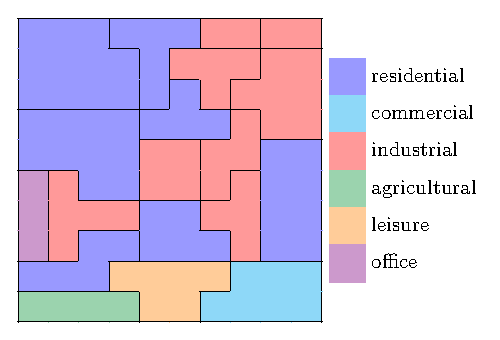
\includegraphics[width=1\linewidth]{images/genetic_algorithm_result_table.pdf}
 \caption{평가 함수를 극대화하는 도시 설계안의 시설과 범주를 나타내는 지도}
 \label{fig:enter-label}
\end{figure}

도시의 설계 목적에 알맞게 hyper parameter를 설정함으로써 다양한 결과를 도출할 수 있다.

도시의 경제적 효과, 그 중에서도 

여기에 사진

경제적 가치 창출량이 높은 공장이 도시의 많은 영역을 차지하도록 결과가 도출된 것을 확인할 수 있다. 반대로 경제적 가치보다 환경친화성에 대한 가중치를 증가시킨 경우, 다음과 같은 시뮬레이션 결과를 얻을 수 있다.

여기에 사진

앞의 결과들과의 비교를 통해 도시의 시설들이 환경 가치가 적은 형식으로 도출되었음을 확인할 수 있다.

\section{결론 및 제언}
\subsection{}

 본 모델로 도출한 최적의 배치는 주거, 사무, 산업 시설로 구성된 전형적인 도시의 개형을 나타낸다. 이는 우리가 살아가고 있는 도시의 형태가 경제적, 사회/문화적, 환경적인 요소와 시설간의 상호작용이 잘 반영되어 있음을 나타낸다. 우리가 설계한 평가함수와 최적 배치 알고리즘은 초기조건을 다르게 설정하여 설계하고자 하는 도시의 상황을 반영할 수 있다는 점에서 의의를 가진다. 설정한 가중치를 도시의 목적에 맞게 수정해가며 범용적으로 사용할 수 있다. 또, 주변 도시나 보전 지역 등 고정된 요소를 설정하여 실제 상황을 반영한 최적화된 도시 계획을 얻을 수 있을 것으로 기대한다.
 
\subsection{}
 시설의 생산 가치를 고려할 때, 건설 효과에 따른 추가 경제적 가치를 포함하여 연구를 개선할 수 있을 것이다. 다지 투산출표(multi-regional IO, MRIO) 자료를 활용하여 새로 건설하고자 하는 도시와 주변 도시의 상호작용을 계산하여\cite{chungnam_technical_report}, 이에 따른 주변 도시의 경제적 효과를 생산가치에 포함하여 더 향상된 평가함수를 구현할 수 있을 것이다.

국가 차원에서 설립한 공공시설의 경우 단순히 WTP를 계산하는 것 외에도, 예산 대비 WTP를 측정하여 ROI 값을 계산하여 가치를 추정할 수도 있다. 위 연구에서는 하나의 평가함수로 통일하는데 용이하도록 가치의 단위를 통일하기 위하여 위 방법은 제외하였다.
 
 특정 산업종에 대한 가중치를 부여하거나 제한적인 인구를 가정하는 등 본 모델의 인자에 적절한 수정을 가하면 특수 목적 도시의 설계나 농촌 개발 사업, 신축 공장의 위치 선정 등 다양한 방면으로 응용할 수 있을 것으로 기대된다.
\section{References}
\printbibliography

\end{multicols}
\end{document}